\chapter{Experiments and results}

\section{Evaluation datasets}

\subsection{Colorchecker}

The ColorChecker dataset is a collection of images for evaluating Color Constancy algorithms built as additional material to \cite{gehler2008bayesian}. It consists in 568 RGB colored images of different scenes, both indoor and outdoor taken under different illuminations. In each scene a Gretag MacBeth Color Checker Chart was placed such that it was illuminated by the main scene illuminant and thus its color could be retrieved. The data is available in Canon RAW format free of any correction.

\begin{figure}[h!]
  \centering
    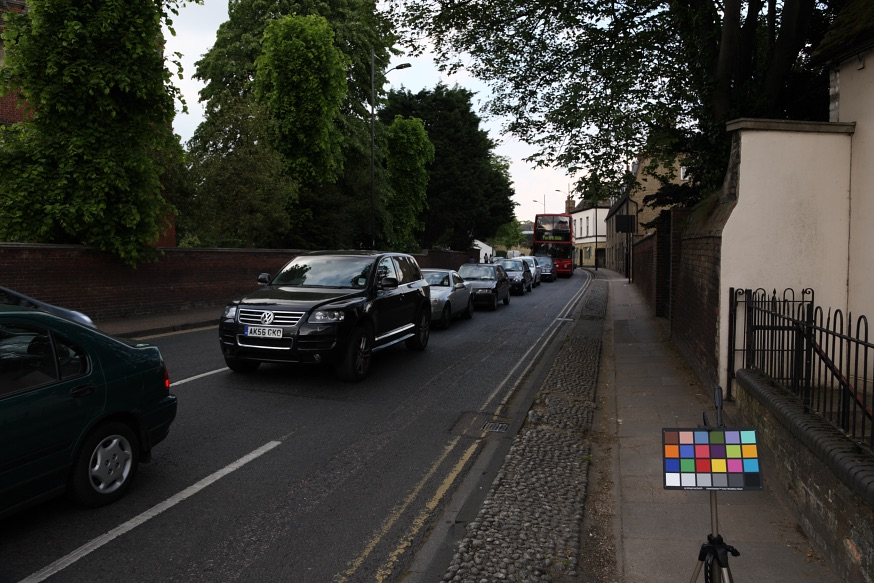
\includegraphics[width=0.65\textwidth]{colorchecker_sample}
    \caption{Example of an image of the ColorChecker dataset}
    \label{fig:colorcheckersample}
\end{figure}

This dataset has been mainly used for experimenting on pristine data: due its characteristics is very varied and lends itself well to image analysis based on color.

\subsection{DSO-1}

The DSO-1 dataset\footnote{Public available for download at https://recodbr.wordpress.com/code-n-data} is composed of 200 indoor and outdoor images with image resolution of 2048 × 1536 pixels. Out of this set of images, 100 are original, i. e., have no adjustments whatsoever, and 100 are forged. 

\begin{figure}[h!]
  \centering
    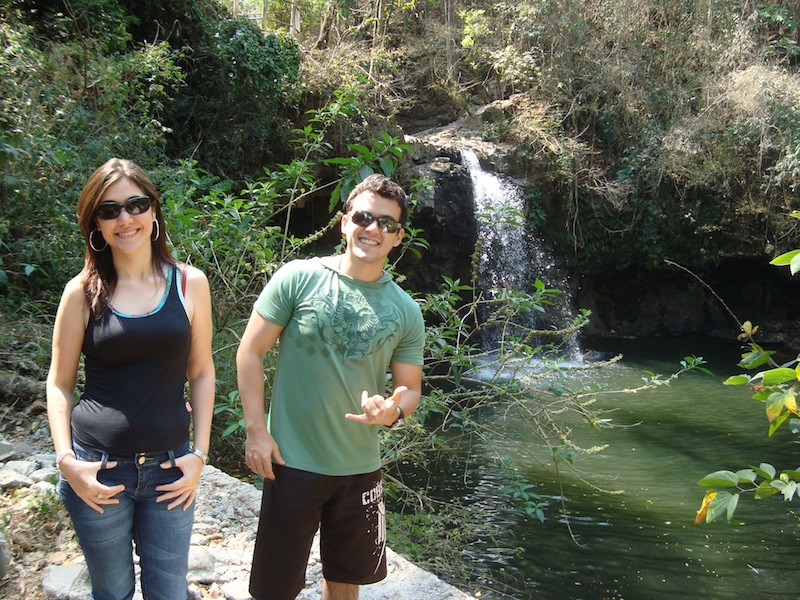
\includegraphics[width=0.65\textwidth]{dso1_sample}
    \caption{Example of an image of the DSO-1 dataset}
    \label{fig:dsosample}
\end{figure}

The forgeries were created by adding one or more individuals in a source image that already contained one or more people. When necessary, we complemented an image splicing operation with post-processing operations (such as color and brightness adjustments) in order to increase photorealism.

\subsection{DSI-1}

The DSI-1 dataset is composed of 50 images (25 original and 25 doctored) downloaded from different websites in the Internet with different resolutions. Original images were downloaded from Flickr and doctored images were collected from different websites such as Worth 1000, Benetton Group 2011, Planet Hiltron, etc.

\begin{figure}[h!]
  \centering
    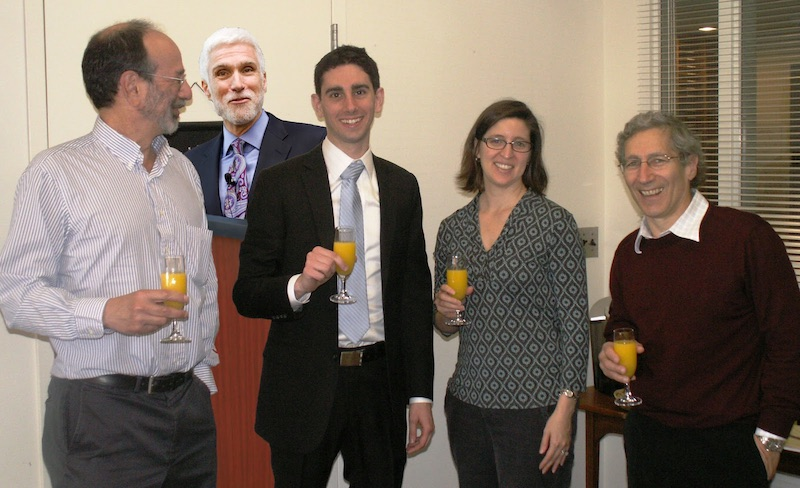
\includegraphics[width=0.65\textwidth]{dsi1_sample}
    \caption{Example of an image of the DSI-1 dataset}
    \label{fig:dsisample}
\end{figure}

\subsection{NIMBLE}

\section{Test cases}

\section{Performance}
